\mychapter{Construção do reconhecedor}
\label{Cap:construcao-reconhecedor}

Nessa etapa foi feita a construção do reconhecedor para a linguagem LazyComb baseado no autômato de pilha estruturado.

\section{Notação BNF}
\label{sec:notacao-bnf}

Linguagem em notação BNF:

\begin{lstlisting}
    <Program>  ::= <CCExpr>     
                    
    <CCExpr>   ::= <CCExpr> <Expr> | epsilon                   

    <Expr>     ::= i | <Expr'>                      

    <IotaExpr> ::= i | <Expr'>

    <Expr'>    ::= I                        
               | K | k                  
               | S | s                               
               | <NonemptyJotExpr           
               | ` <Expr1> <Expr2>            
               | * <IotaExpr1> <IotaExpr2>    
               | ( <CCExpr> )             

    <NonemptyJotExpr> ::= <JotExpr> 0                
                        | <JotExpr> 1                

    <JotExpr>  ::= <NonemptyJotExpr> | epsilon

\end{lstlisting}

\section{Notação Wirth}

A partir da notação em BNF, foi obtida a notação em Wirth:

\begin{lstlisting}
    Program     = CCExpr.     
                    
    CCExpr      = { Expr }.                  

    Expr        = "i" | Expr'                      

    IotaExpr    = "i" | Expr'

    Expr'    ::= "I"                        
               | "K" | "k"                  
               | "S" | "s"                               
               | NonemptyJotExpr           
               | "`" Expr Expr       
               | "*" IotaExpr IotaExpr    
               | "(" CCExpr ")"             

    NonemptyJotExpr ::= JotExpr "0"                
                        | JotExpr "1"     

    JotExpr = NonemptyJotExpr | epsilon.           
\end{lstlisting}

\section{Análise Léxica}

Como todos os terminais da linguagem são compostos apenas por um caracter, a tarefa do analisador léxico se torna simples, basta verificar se a entrada está contida no conjunto de caracteres válidos.

\begin{figure}[H]
\centering
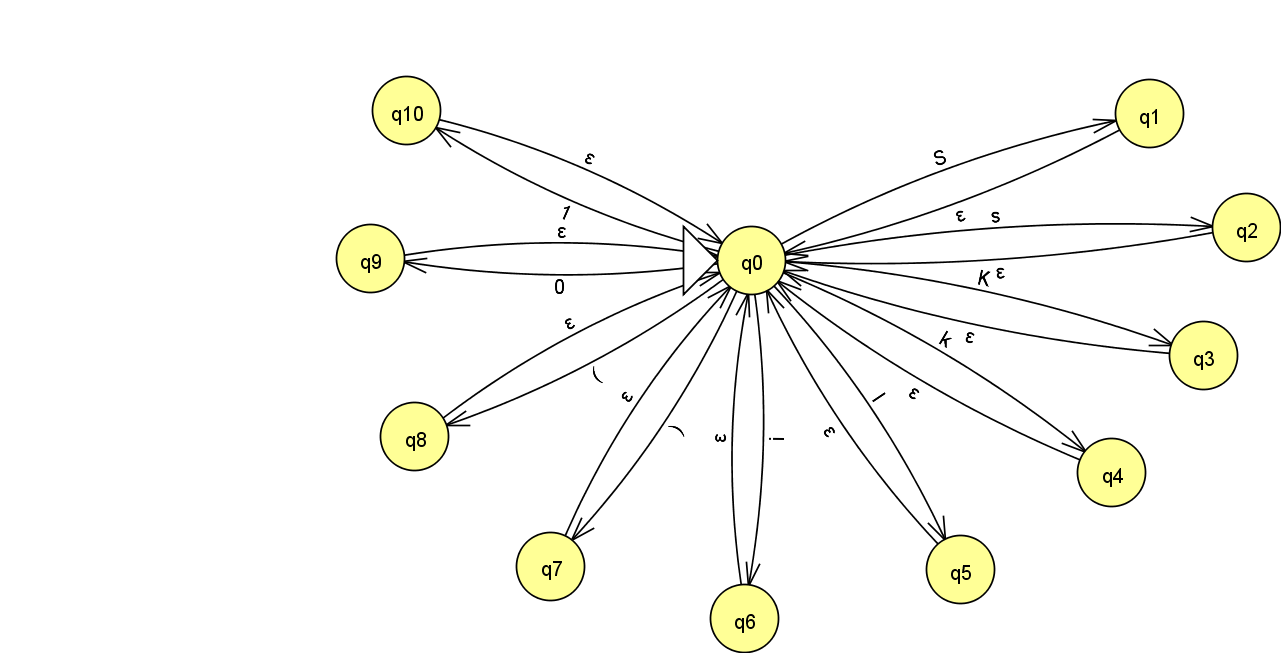
\includegraphics[width=14cm,keepaspectratio]{jflap-automatas/lexico.png}
\caption{\label{fig:jflap-lexico} Transdutor - Analisador léxico}
\end{figure}

\section{Análise Sintática}

A partir da notação em Wirth, foi feita uma simplificação:

\begin{lstlisting}
    Program = { Expr }.

    Expr = "i" | "I" | "K" | "k" | "S" | "s" | { "0" | "1" } | "`" Expr Expr | "*" IotaExpr IotaExpr | "(" { Expr } ")".
    
    IotaExpr = "i" | "I" | "K" | "k" | "S" | "s" | { "0" | "1" } | "`" Expr Expr | "*" IotaExpr IotaExpr | "(" { Expr } ")".
\end{lstlisting}

Para cada não terminal foi gerada uma máquina sintática, representada pelos seu estado inicial, estados finais e  transições entre estados. Cada transição pode se manifestar na forma de chamada ou retorno para uma submáquina, ou execução de uma ação semântica, tudo isso usando autômato de pilha estruturado (empilhando ou desempilhando máquinas).

Utilizando o site http://mc-barau.herokuapp.com/ e o programa JFLAP, a descrição da linguagem em notação de Wirth resultou nas seguintes máquinas:

\subsubsection{Program}

\begin{lstlisting}
Program = 0 { 1 Expr 2 } 1 .

Program: 
Minimized DFA: 
initial: 0
final: 1
(0, Expr) -> 1
(1, Expr) -> 1       
\end{lstlisting}

\begin{figure}[H]
\centering
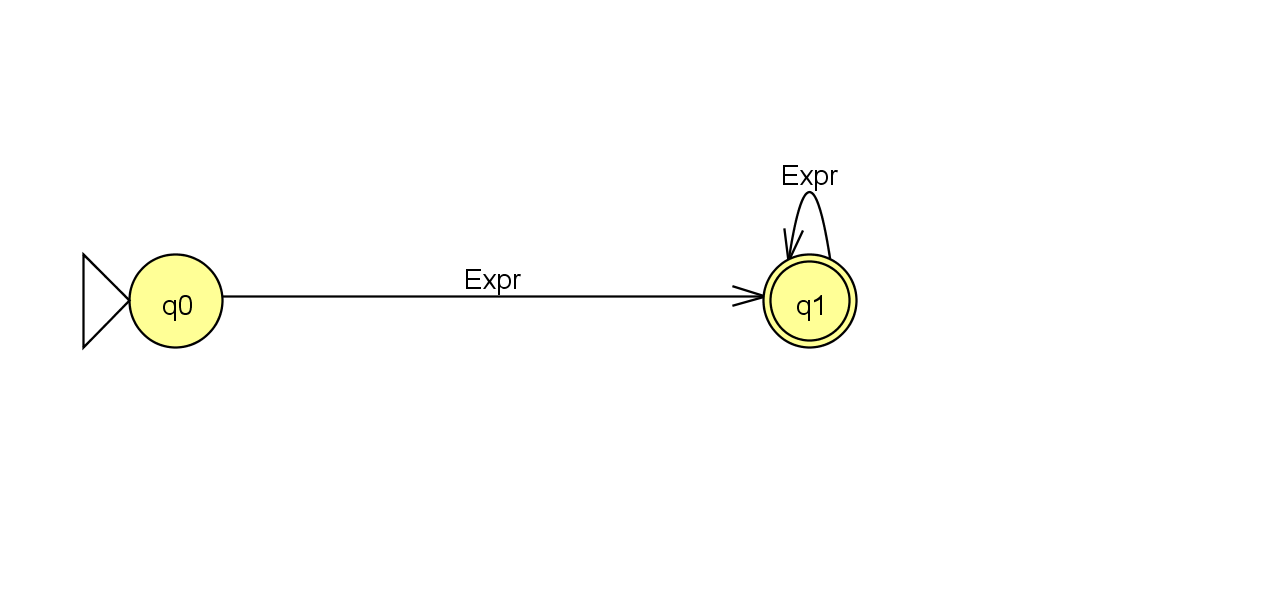
\includegraphics[width=15cm,keepaspectratio]{jflap-automatas/program.png}
\caption{\label{fig:jflap-program} Program}
\end{figure}

\subsubsection{Expr}

\begin{lstlisting}  
Expr = 0 "i" 1 | 0 "I" 2 | 0 "K" 3 | 0 "k" 4 | 0 "S" 5 | 0 "s" 6 | 0 { 7 "0" 8 | 7 "1" 9 } 7 | 0 "`" 10 Expr 11 Expr 12 | 0 "*" 13 IotaExpr 14 IotaExpr 15 | 0 "(" 16 { 17 Expr 18 } 17 ")" 19 .
                   
Sub-maquina Expr: 
Minimized DFA: 
initial: 0
final: 1, 2
(0, "i") -> 1
(0, "I") -> 1
(0, "K") -> 1
(0, "k") -> 1
(0, "S") -> 1
(0, "s") -> 1
(0, "0") -> 2
(0, "1") -> 2
(0, "`") -> 3
(0, "*") -> 4
(0, "(") -> 5
(2, "0") -> 2
(2, "1") -> 2
(3, Expr) -> 7
(4, IotaExpr) -> 6
(5, Expr) -> 5
(5, ")") -> 1
(6, IotaExpr) -> 1
(7, Expr) -> 1
\end{lstlisting}

\begin{figure}[H]
\centering
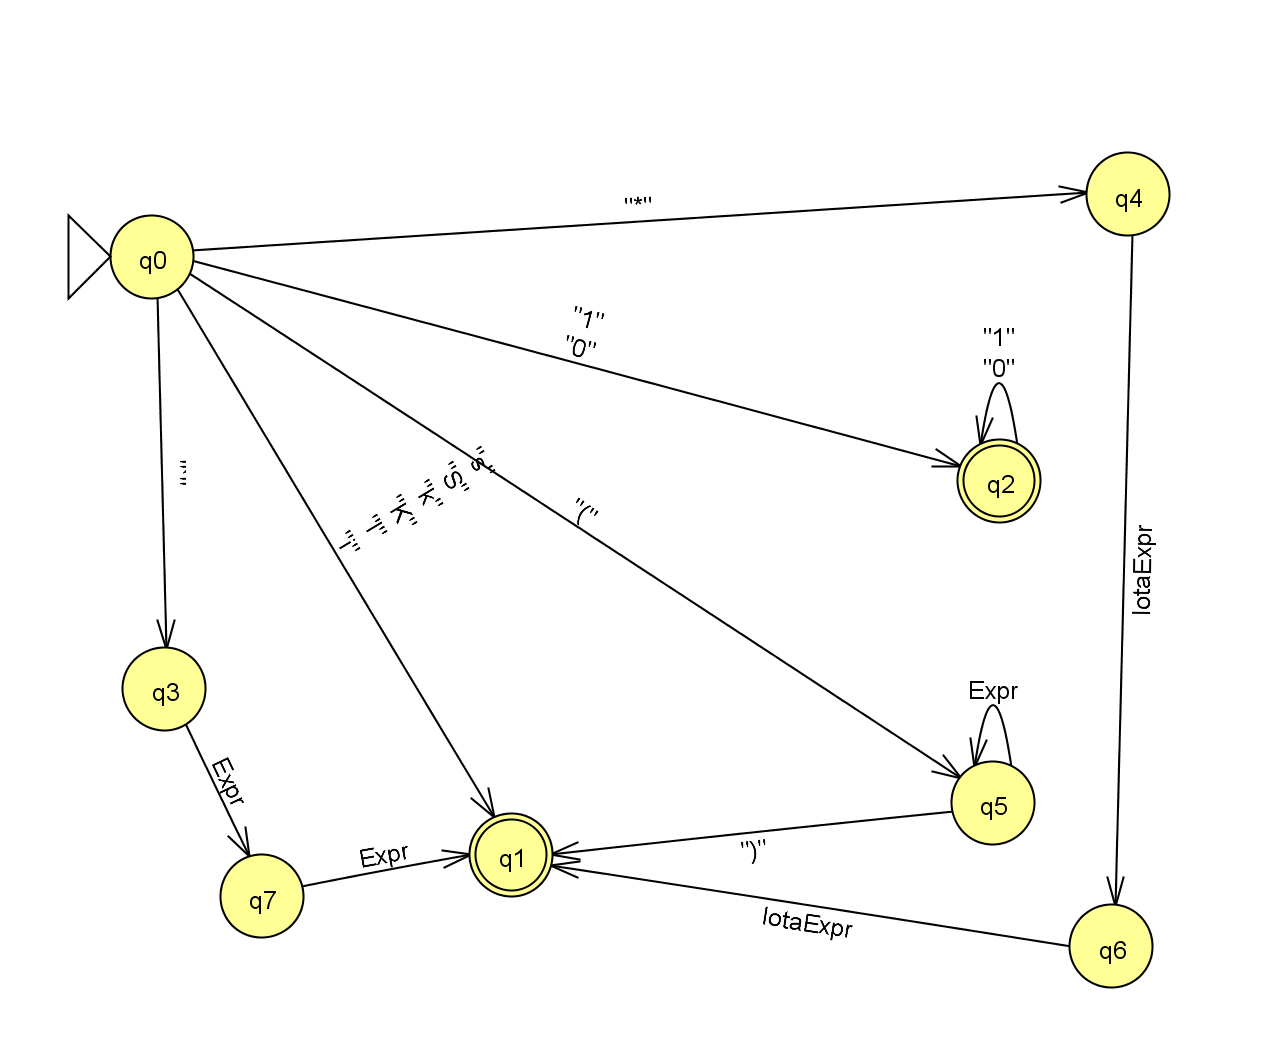
\includegraphics[width=15cm,keepaspectratio]{jflap-automatas/expr.png}
\caption{\label{fig:jflap-expr} Expr}
\end{figure}

\subsubsection{IotaExpr}

\begin{lstlisting}  
IotaExpr = 0 "i" 1 | 0 "I" 2 | 0 "K" 3 | 0 "k" 4 | 0 "S" 5 | 0 "s" 6 | 0 { 7 "0" 8 | 7 "1" 9 } 7 | 0 "`" 10 Expr 11 Expr 12 | 0 "*" 13 IotaExpr 14 IotaExpr 15 | 0 "(" 16 { 17 Expr 18 } 17 ")" 19 .
            
Sub-maquina IotaExpr: 
Minimized DFA: 
initial: 0
final: 1, 2
(0, "i") -> 1
(0, "I") -> 1
(0, "K") -> 1
(0, "k") -> 1
(0, "S") -> 1
(0, "s") -> 1
(0, "0") -> 2
(0, "1") -> 2
(0, "`") -> 3
(0, "*") -> 4
(0, "(") -> 5
(2, "0") -> 2
(2, "1") -> 2
(3, Expr) -> 7
(4, IotaExpr) -> 6
(5, Expr) -> 5
(5, ")") -> 1
(6, IotaExpr) -> 1
(7, Expr) -> 1
\end{lstlisting}

\begin{figure}[H]
\centering
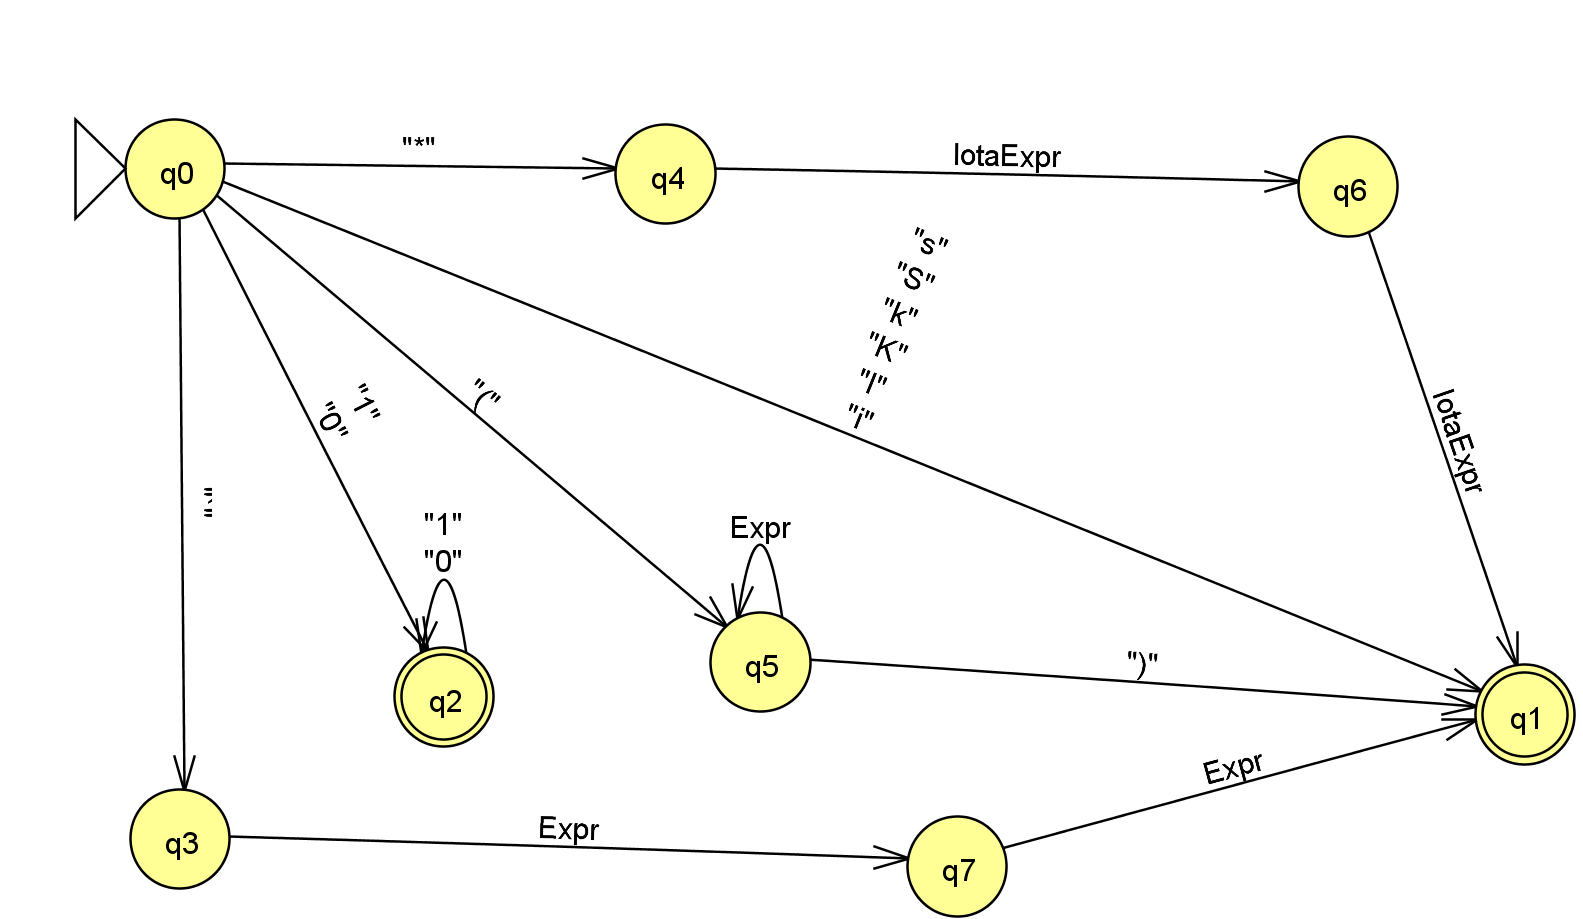
\includegraphics[width=15cm,keepaspectratio]{jflap-automatas/iotaexpr.png}
\caption{\label{fig:jflap-iotaexpr} IotaExpr}
\end{figure}